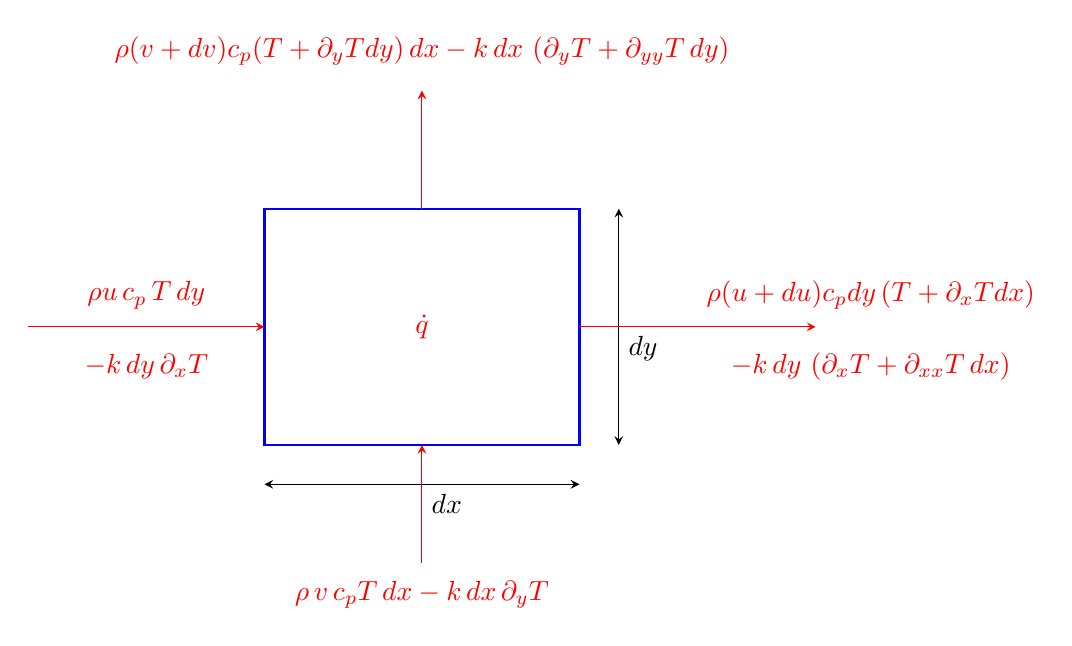
\begin{tikzpicture}[>=stealth]
    % Define convenient lengths for dx and dy
    \def\dx{4}
    \def\dy{3}
    
    % Draw the control-volume rectangle
    \draw[thick, blue] (0,0) rectangle (\dx,\dy);
    
    % Label dx and dy
    \draw[<->] (0,-0.5) -- (\dx,-0.5) node[midway,below right] {$dx$};
    \draw[<->] (\dx+0.5,0) -- (\dx+0.5,\dy) node[midway,below right] {$dy$};
    
    % Left edge - energy in
    \draw[red, ->] (-3,\dy/2) -- (0,\dy/2);
    \node[red, align=left] at (-1.5,\dy/2+0.4) {$\rho u\,c_p\,T\,dy $};
    \node[red, align=left] at (-1.5,\dy/2-0.5) {$-k\,dy \, \partial_x T$};
    
    % Right edge - energy out
    \draw[red, ->] (\dx,\dy/2) -- (\dx+3,\dy/2);
    \node[red, align=left] at (\dx+3.7,\dy/2+0.4) {$\rho(u + du)c_p dy \left(T + \partial_x T dx\right) $};
    \node[red, align=left] at (\dx+3.7,\dy/2-0.5) {$-k\,dy\, \left(\partial_x T + \partial_{xx} T \,dx\right)$};
    
    % Bottom edge - energy in
    \draw[red, ->] (\dx/2,-1.5) -- (\dx/2,0);
    \node[red, align=center] at (\dx/2,-1.9) {$\rho\, v\,c_p T\,dx - k\,dx \,\partial_y T$};
    
    % Top edge - energy out
    \draw[red, ->] (\dx/2,\dy) -- (\dx/2,\dy+1.5);
    \node[red, align=center] at (\dx/2,\dy+2.0) {$\rho(v + dv)c_p(T + \partial_y T dy)\,dx -k\,dx\, \left(\partial_y T + \partial_{yy} T \,dy \right)$};
    
    % Heat generation in the center
    \node[red] at (\dx/2,\dy/2) {$\dot{q}$};
    
\end{tikzpicture}